\subsubsection{Brisanje naloga usled raskida ugovora na zahtev snabdevača}

\begin{itemize}
    \item Kratak opis:
        \begin{itemize}
            \item Snabdevač briše nalog i inicira raskid ugovora.
        \end{itemize}
    \item Učesnici:
        \begin{itemize}
            \item Administrator
            \item Snabdevač
        \end{itemize}
    \item Preduslovi:
        \begin{itemize}
          \item Sistem je u funkciji.
            \item Snabdevač mora da bude registrovan i prijavljen na sistem.
            
        \end{itemize}
    \item Postuslovi:
        \begin{itemize}
            \item Uspešno je raskinut ugovor između snabdevača i HelloFresh kompanije.
            \item Snabdevač prestaje se uslugom dostavljanja namirnica.
            \item Nalog snabdevača je obrisan iz sistema.
        \end{itemize}
    \item Osnovni tok:
        \begin{enumerate}
            \item Snabdevač pristupa veb stranici i bira opciju za brisanje naloga.
            \item Sistem izbacuje upozerenje o brisanju naloga i traži od snabdevača da unose šifru ako želi da nastavi.
            \item Snabdevač potvrdjuje da je siguran da želi da obriše nalog tako što ponovo unosi svoju šifru.
            \item Sistem proverava šifru, obrađuje zahtev za raskid ugovora i obaveštava administratora.
            \item Administrator obavlja razgovor sa snabdevačem i vrši raskid ugovora.
            \item Sistem uklanja snabdevača iz spiska dostupnih snabdevača i iz sistema.
        \end{enumerate}
    \item Alternativni tok:
        \begin{itemize}
            \item[2.a] Snabdevač odustaje od brisanja naloga. Slučaj upotrebe se završava.
            \item[4.a] Snabdevač nije ukucao tačnu šifru. Slučaj upotrebe se nastavlja od koraka 2.
        \end{itemize}
\end{itemize}

\begin{figure}[H]
\begin{center}
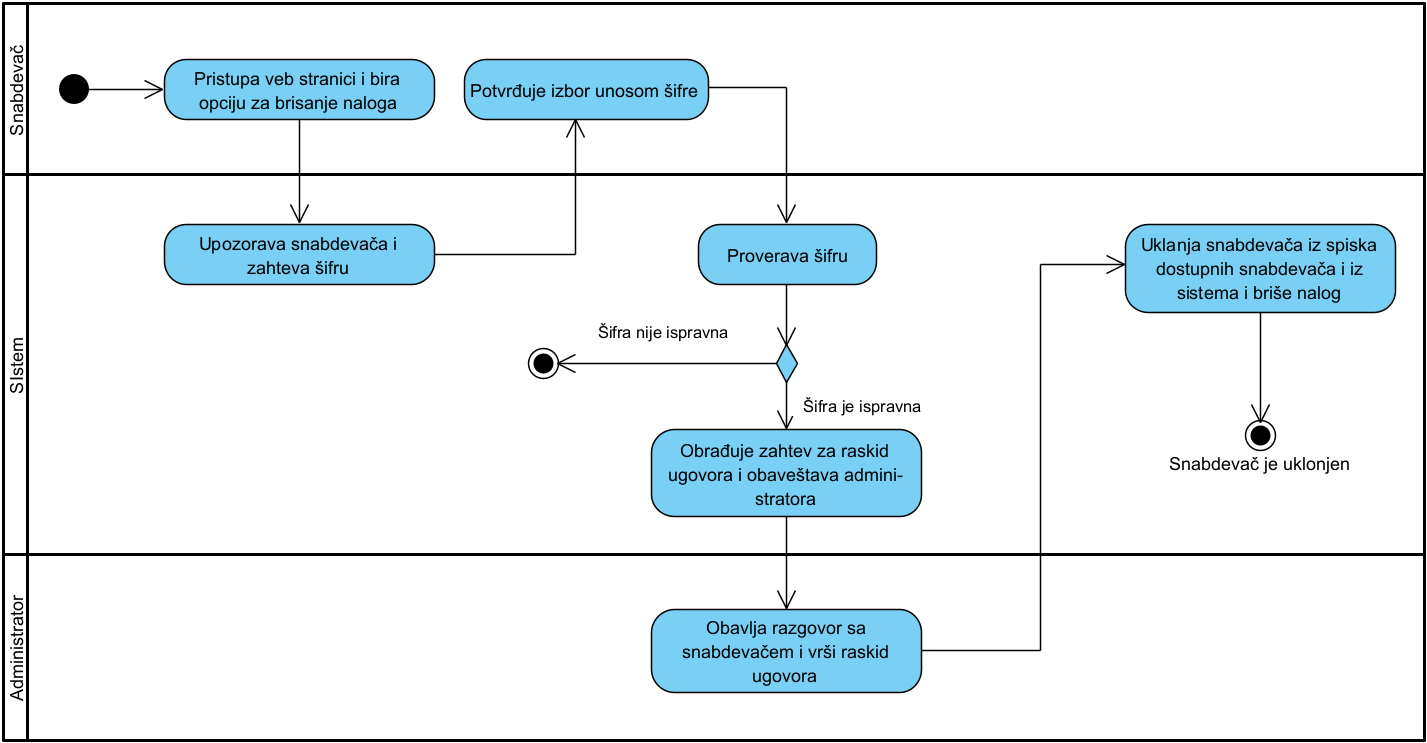
\includegraphics[width=\textwidth]{Pictures/activity_supplier_contract_termination_1.png}
\end{center}
    \caption{Dijagram aktivnosti raskida ugovora na zahtev snabdevača}
\label{fig:ActivitySupplierContractTermination1}
\end{figure}

\subsubsection{Brisanje naloga usled raskida ugovora na zahtev HelloFresh kompanije}

\begin{itemize}
    \item Kratak opis:
        \begin{itemize}
            \item Administrator inicira raskid ugovora sa snabdevačem i briše njegov nalog.
        \end{itemize}
    \item Učesnici:
        \begin{itemize}
            \item Administrator
        \end{itemize}
    \item Preduslovi:
        \begin{itemize}
            \item Postoji snabdevač koje je registrovan a prekršio neku od klauzula ugovora.
            \item Sistem je u funkciji.
        \end{itemize}
    \item Postuslovi:
        \begin{itemize}
            \item Uspešno je raskinut ugovor između snabdevača i HelloFresh kompanije.
            \item Snabdevač prestaje se uslugom dostavljanja namirnica.
            \item Nalog snabdevača je uklonjen iz sistema.
        \end{itemize}
    \item Osnovni tok:
        \begin{enumerate}
            \item Administrator uočava da je snabdevač prekršio uslove ugovora.
            \item Administrator vrši raskid ugovora i obaveštava snabdevača o raskidu.
            \item Sistem uklanja snabdevača iz spiska dostupnih snabdevača i iz sistema.
        \end{enumerate}
\end{itemize}

\begin{figure}[H]
\begin{center}
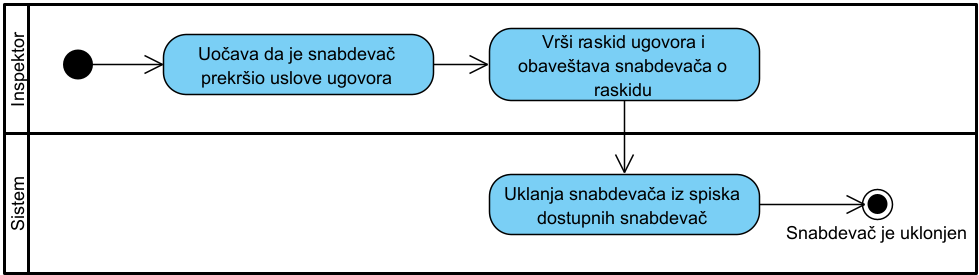
\includegraphics[width=\textwidth]{Pictures/activity_supplier_contract_termination_2.png}
\end{center}
    \caption{Dijagram aktivnosti raskida ugovora na zahtev HelloFresh komapanije}
\label{fig:ActivitySupplierContractTermination2}
\end{figure}